\subsection{ソフトウェアエンジニアリング運用提供}

運用提供は、計画された運用サービスを実際に実行し、ソフトウェアを本番利用に耐える形で届ける活動である。ここでは、運用テスト、配備、リリース、ロールバック、データ移行、問題解決が中心となる。

\subsubsection{運用テスト、検証、受け入れ}

運用テストは、ソフトウェアが本番環境または本番に近い環境で運用可能かを確認する活動である。検証は「仕様どおりか」を確認する活動であり、受け入れは「利用者や運用者が使えると判断できるか」を確認する活動である。

現代の運用では、テストは最後に一回だけ行うものではない。テスト駆動開発（TDD）や受け入れテスト駆動開発（ATDD）を使い、開発中から継続的に検証を行う。DevOpsでは、試験サービスや試験ツールを自動化し、開発者が変更のたびに素早く結果を得られるようにする。

\subsubsection{配備・リリース工学}

配備とは、指定された版のソフトウェアを、特定の環境へインストールすることである。リリースとは、機能または機能集合を、顧客や利用者が実際に使える状態にすることである。配備とリリースは似ているが、同じではない。配備は技術的な配置であり、リリースは利用可能にする判断である。

\par\smallskip\noindent\refstepcounter{table}\label{tab:ch06-06}\textbf{表 \thetable: 第06章 ソフトウェアエンジニアリング運用 表06}\par\smallskip
\begin{longtable}{L{35mm}L{115mm}}
\toprule
概念 & 説明 \\
\midrule
配備 & コード、設定、データベース、サーバ、コンテナなどを対象環境へ置き、動作可能にする技術的活動である。 \\
リリース & 配備済みの機能を、すべての利用者または一部の利用者に使えるようにする活動である。ビジネス判断を含む。 \\
\bottomrule
\end{longtable}

従来は、開発チームが完成物を運用チームに引き渡し、運用チームが手作業で配備することが多かった。この方法は時間がかかり、品質面でもリスクがある。DevOpsでは、コードの包装、設定ファイル生成、サーバ再起動、サーバとデータベースの設定、ソフトウェアのインストール、アプリケーション起動、スモークテストを自動化する。

リリース戦略には、環境に基づく戦略とアプリケーションに基づく戦略がある。環境に基づく戦略では、新版を事前本番環境や別環境へ配備してから切り替える。アプリケーションに基づく戦略では、機能トグルのような設定により、コード中の特定機能を有効化または無効化する。

カナリアリリースは、変更を一部の範囲にだけ短期間配備し、その結果を評価してから全面配備を判断する方法である。新しいソフトウェアが異常を示した場合、自動的にロールバックできる構成も重要である。

\begin{figure}[htbp]
\centering
\IfFileExists{assets/generated_figures/ch06/fig-ch06-07.png}{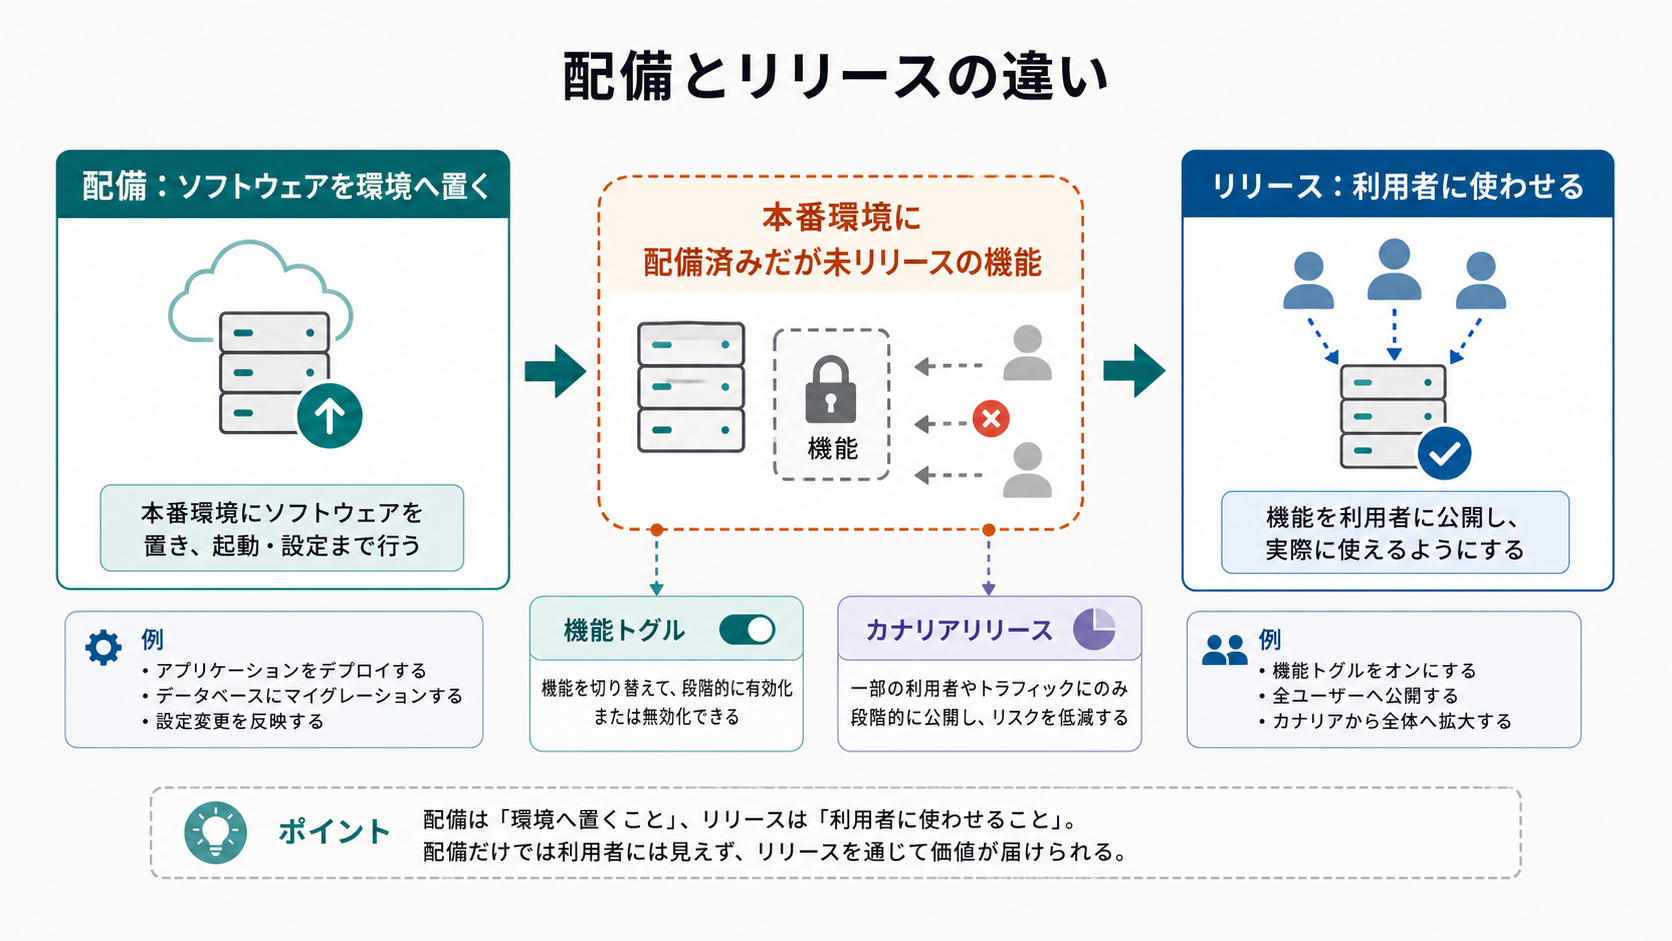
\includegraphics[width=0.96\linewidth]{assets/generated_figures/ch06/fig-ch06-07.png}}{\fbox{\parbox[c][48mm][c]{0.9\linewidth}{\centering 画像生成待ち\\配備とリリースの違い}}}
\caption{配備とリリースの違い}
\label{fig:ch06-07}
\end{figure}

\subsubsection{ロールバックとデータ移行}

ロールバックとは、新しい版のソフトウェアやデータベースが問題を起こしたとき、正しく動く以前の状態へ戻す活動である。データ移行とは、ソフトウェア変更に合わせてデータ構造や内容を移す活動である。

本番配備前には、ロールバック手順が計画され、練習されるべきである。新しい版が障害や性能劣化を起こした場合、素早く以前の状態へ戻せる必要がある。DevOpsでは、この過程を自動化し、監視結果に応じて自動的に戻すことも可能である。

データ移行がある場合、単にプログラムを戻すだけでは不十分である。データの形式が変わっていると、旧版が新しいデータを読めないことがある。したがって、ロールバック計画には、データをどの状態に戻すか、どこまでの処理を再実行するか、利用者にどの影響があるかを含める必要がある。

\begin{figure}[htbp]
\centering
\IfFileExists{assets/generated_figures/ch06/fig-ch06-08.png}{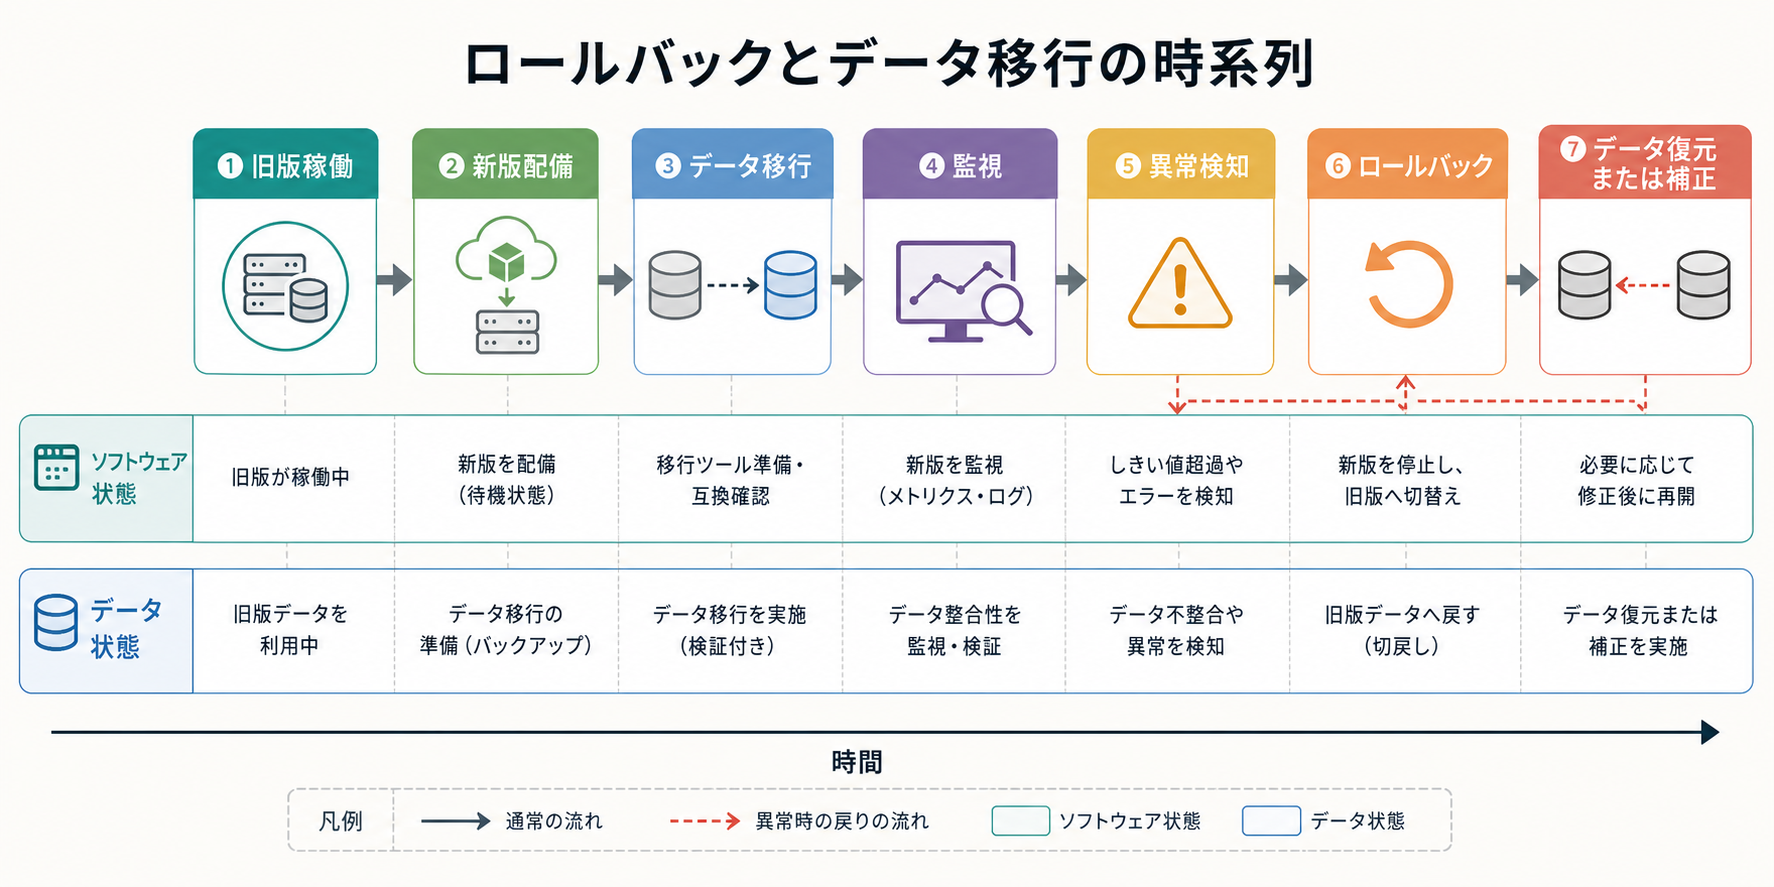
\includegraphics[width=0.96\linewidth]{assets/generated_figures/ch06/fig-ch06-08.png}}{\fbox{\parbox[c][48mm][c]{0.9\linewidth}{\centering 画像生成待ち\\ロールバックとデータ移行の時系列}}}
\caption{ロールバックとデータ移行の時系列}
\label{fig:ch06-08}
\end{figure}

\subsubsection{問題解決}

問題解決は、ソフトウェアやシステムのインシデントと問題の原因を識別し、分析し、事業への混乱を最小化する活動である。繰り返し発生する本番問題には、ソフトウェア、インフラ、設定、データベース、ネットワーク、人間の手順など、複数の原因が絡むことがある。そのため、問題解決には、ソフトウェア技術者、運用担当技術者、セキュリティ担当、データベース担当、製品責任者などの多職種チームが必要になる場合がある。

問題解決では、監視、ログ、プロファイル、実行トレース、設定履歴を使って、何が起きたか、いつ起きたか、どの変更と関係するかを調べる。問題の根本原因がわかれば、再発防止策を実装する。
